\documentclass{article}

\usepackage{kafkanotes}

%Judul dan Penulis
\title{Lecture Notes on Quatum Mechanics}
\author{Daniel David Torres Amaris}

\begin{document}

%Halaman Judul
\begin{titlepage}
\thispagestyle{empty}
\maketitle

%Abstrak
\begin{abstract}
Lecture notes on Quatum Mechanics for 2024-2 course helded in the Universidad de Pamplona. This document consists mainly of a compilation of my notes after studying the book of Sakurai along with the exercices and examples that I used along the course.
\end{abstract}

\tableofcontents
\end{titlepage}

\newgeometry{top=20mm,bottom=25mm,right=80mm,left=20mm}


\section{Introduction}
Before quatum mechanics, everithing was explained in terms of particles and waves, separated worlds whose interacting was described by the Lorentz force or by thermodynamics. Only relativistic and microscopic systems were out of reach for Newtonian physics. Atomic stability, atomic spectra, the photoelectric effect and black body radiation where the final problems of physics. Quantum mechanics has its origins on the attemp to explain the differences observed between the emision spectra of gases and a black body. The first showed a discrete behavior while latter turned out continuous. A black body (see fig. \ref{fig:blackbodyimg}) consists of a system emmits the same amount of energy that it absorbs; a real life realization of a black body can be achieved by metallic box with perfectly reflectant wall and one hole. In such a system, the hole behaves as a black body, absorbing all the wavelengths and emmiting all of them after multiple reflection over the inner part of the box. Thus, a black body is a perfect absorber and a perfect emmiter.
\begin{marginfigure}%
  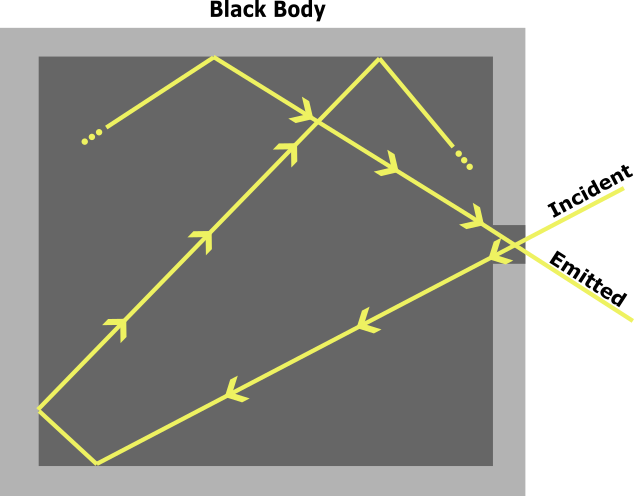
\includegraphics[width=\linewidth]{figures/blackbodyimg}
  \caption{Physical realization of a black body.}
  \label{fig:blackbodyimg}
\end{marginfigure}
Besides this notorious differences, further difficulties arose from the very descripton of the black body radiation. Experimental measurements performed on a variety of black bodies made out of different materials showed energy distributions with zero radiance for the 0 nm wavelenth, then increasing until a maximum after which the radiance decreases monotonically until it becomes vanishingly small for large wavelenths. The solid curve in fig. \ref{fig:blackbodyrad} depicts the mentioned behavior.
\begin{marginfigure}%
  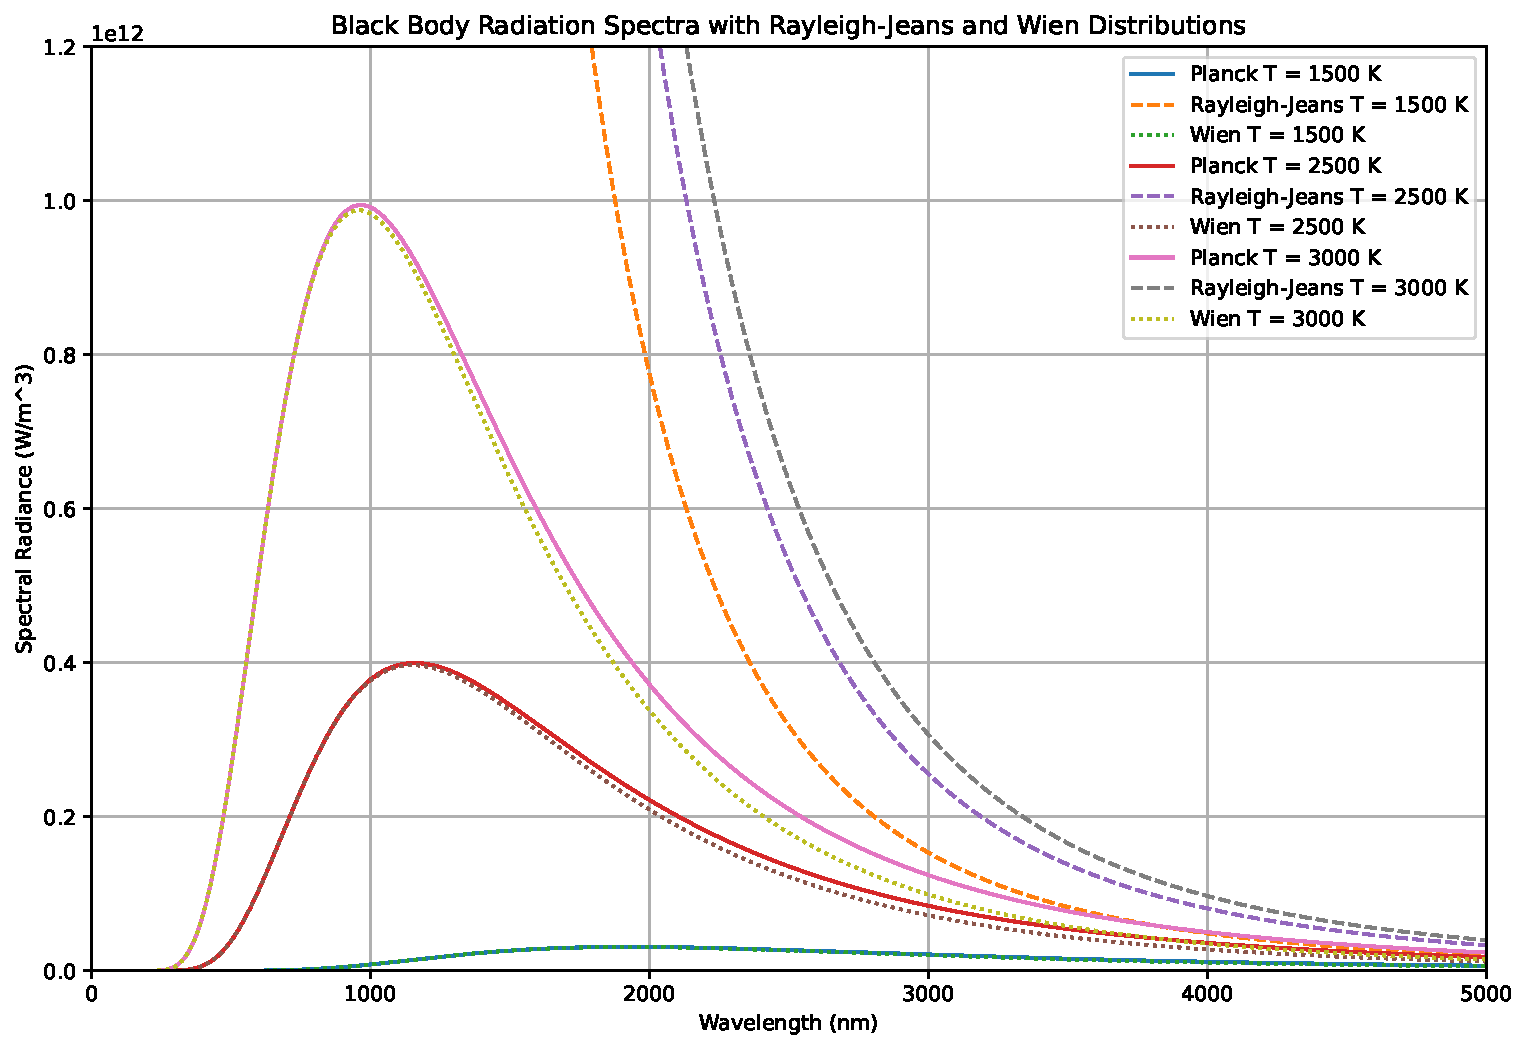
\includegraphics[width=\linewidth]{figures/blackbody}
  \caption{Black body radiance distribution.}
  \label{fig:blackbodyrad}
\end{marginfigure}
Attempts to describe the observed behavior where made by Wien and by Rayleigh (see doted and dashed plots respectively in fig. \ref{fig:blackbodyrad}). The Wien's law, derived the spectral radiance $u(\lambda,T)$ from the thermodynamic point of view, achieves a good approximation for small wavelenghts and discrepancies for high wavelenghts, according to the following equation
\begin{equation}
  u(\lambda, T) = \frac{2hc^2}{\lambda^5} e^{-\frac{hc}{\lambda k_\text{B} T}},
\end{equation}
where $\lambda$ is the wavelength, T is the temperature in Kelvin, $h$, $k_B$ and $c$ are the Planck's, Boltzmann's and the speed of light constants.
The Rayleigh-Jeans distribution, derived from statistics considering the cavity full of standing waves at equilibrium and usign the equipartition theorem, arrived to a clear imposibility where the system can have an infinite total energy and infinite radiance is allowed for small wavelenghts! 
\begin{equation}
  u(\lambda,T) = \frac{2ck_\text{B}T}{\lambda^4}.
\end{equation}
Planck in an attemp to improve the fitting of the Wien's distribution used a similar procedure than Rayleigh's. Thus, starting from the average energy for the harmonic oscillators inside the cavity
\begin{equation}\label{eq:equipart}
  <E> = \frac{\int_0^\infty E e^{-E/k_B T}dE}{\int_0^\infty e^{-E/k_B T}dE},
\end{equation}
but postulating discrete emitting harmonic oscillators allowed only to emit energy in multiples of $h\nu$,
\begin{equation}
  E = nh\nu, n=0,1,2,...
\end{equation}
he was able to change the integral in eq. \ref{eq:equipart} for a sumation as follows
\begin{equation}\label{eq:planckequipart}
  <E> = \frac{\sum_{n=0}^\infty nh\nu e^{-nh\nu/k_B T}}{\sum_{n=0}^\infty e^{-nh\nu/k_B T}} = \frac{h\nu}{e^{\frac{h\nu}{k_B T}}-1}.
\end{equation}
Multiplying eq \ref{eq:planckequipart} by the number of modes allowed inside the cavity, we have:
\begin{equation}\label{eq:planckrad}
  u(\nu,T) = \frac{8\pi\nu^2}{c^3} \frac{h\nu}{e^{\frac{h\nu}{k_B T}}-1}.
\end{equation}
Notice that you can find the Wien's and Rayleigh's distributions in terms of the frequency by using the substitution $\lambda^{-1}=\frac{\nu}{c}$. This calculation is left as an exercice for the student.
Direct integration of eq. \ref{eq:planckrad} over all the whole spectrum gives
\begin{equation}\label{eq:plancktotal}
  E_{Total} = \int_{0}^{\infty}u(\nu,T)d\nu = \frac{8\pi h}{c^3} \int_0 ^{\infty} \frac{\nu^3}{e^{\frac{h\nu}{k_B T}}-1}=\frac{8\pi^5k_B ^4}{15h^3 c^3}T^4=\frac{4}{c}\sigma T^4,
\end{equation}
where $\sigma$ is the Stefan-Boltzmann constant. In eq. \ref{eq:plancktotal} the total energy is not longer infinite but always depending on the temperature as expected. Furthermore, eq. \ref{eq:planckrad} fitted perfectly with the experimental data. Thus, Planck's distribution for black body radiation solved both the ultraviolet catastrophe and worked seamlessly both in the low and high frequency ranges. All thanks to the discretization imposed over the energy emitted by the oscillators. 
In what follows, we are going to see how this idea was taken by other scientists to solve the remaining problems.
\subsection{Exercices}
Calculate the number of modes allowed inside a cubic cavity of volume v=$a^3$ 
% Proin convallis interdum libero a sollicitudin. In dignissim quam id viverra congue. Pellentesque eget magna massa. Quisque sit amet sagittis felis. Proin a ipsum quis magna sodales egestas non euismod turpis. Sed nisi purus, vestibulum vitae volutpat auctor, euismod sit amet mauris. 

% \begin{margintable}
% \centering
% \begin{tabular}{||c c c c||} 
%  \hline
%  Col1 & Col2 & Col2 & Col3 \\ [0.5ex] 
%  \hline\hline
%  1 & 6 & 87837 & 787 \\ 
%  2 & 7 & 78 & 5415 \\
%  3 & 545 & 778 & 7507 \\
%  4 & 545 & 18744 & 7560 \\
%  5 & 88 & 788 & 6344 \\ [1ex] 
%  \hline
% \end{tabular}
% \captionsetup{justification=centering}
% \caption{Table to test captions and labels}
% \end{margintable}

% Aenean neque mauris, consectetur luctus lacinia vel, viverra a magna. Donec rhoncus venenatis hendrerit.

% \subsection{Subsection with table}
% Lorem ipsum dolor sit amet, consectetur adipiscing elit. Proin sit amet augue sollicitudin, eleifend risus non, scelerisque elit. In tempus dictum nisl nec convallis. Fusce congue, lacus ut mattis lacinia, nulla dolor ultricies sem, eu molestie velit quam et felis. Fusce mattis, dolor vel cursus egestas, tortor nibh efficitur tortor, eget venenatis velit orci ut est. Praesent a diam leo. Vestibulum consectetur vel augue sit amet facilisis. Etiam vitae lorem ut lectus tincidunt feugiat. Interdum et malesuada fames ac ante ipsum primis in faucibus. Nullam sem nulla, posuere sed felis ut, porttitor sagittis lorem. Nam lacus mi, laoreet non fringilla a, eleifend eget turpis. Maecenas ultricies aliquam felis. 

% Lorem ipsum dolor sit amet, consectetur adipiscing elit. Proin sit amet augue sollicitudin, eleifend risus non, scelerisque elit. In tempus dictum nisl nec convallis. Fusce congue, lacus ut mattis lacinia, nulla dolor ultricies sem, eu molestie velit quam et felis. Fusce mattis, dolor vel cursus egestas, tortor nibh efficitur tortor, eget venenatis velit orci ut est. Praesent a diam leo. Vestibulum consectetur vel augue sit amet facilisis. Etiam vitae lorem ut lectus tincidunt feugiat. Interdum et malesuada fames ac ante ipsum primis in faucibus. Nullam sem nulla, posuere sed felis ut, porttitor sagittis lorem. Nam lacus mi, laoreet non fringilla a, eleifend eget turpis. Maecenas ultricies aliquam felis. 

% \subsection{Side figure}

% \begin{marginfigure}%
%   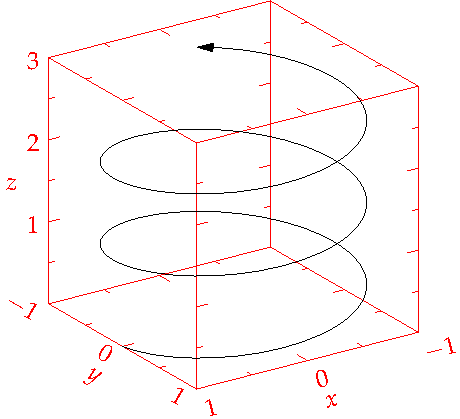
\includegraphics[width=\linewidth]{figures/helix}
%   \caption{This is a margin figure.  The helix is defined by 
%     $x = \cos(2\pi z)$, $y = \sin(2\pi z)$, and $z = [0, 2.7]$.  The figure was
%     drawn using Asymptote (\url{http://asymptote.sf.net/}).}
%   \label{fig:marginfig}
% \end{marginfigure}

% In hac habitasse platea dictumst. Sed elementum pellentesque justo at ultricies. Nunc dapibus nisl nec massa sollicitudin commodo. Nulla sagittis neque ex, in dictum tellus ultricies ut. Integer vulputate metus id ligula efficitur rutrum. Etiam ut est et neque feugiat egestas. Integer ac lacinia urna. 
% Nullam enim nisl, venenatis at luctus malesuada, ultricies rutrum tortor. Aliquam ut nulla congue, pharetra magna vitae, sollicitudin mi. Vestibulum mattis imperdiet sapien ac ornare. In id sagittis sem. Nunc luctus ex sit amet eros posuere viverra. Praesent tristique arcu sed urna rhoncus, vitae aliquam libero mollis. Proin condimentum purus congue arcu mattis sodales. Suspendisse ullamcorper vulputate egestas. Mauris placerat venenatis urna in feugiat. Morbi dignissim arcu nunc. Cras imperdiet neque neque, vel posuere lorem elementum at. 
% In hac habitasse platea dictumst. Sed elementum pellentesque justo at ultricies. Nunc dapibus nisl nec massa sollicitudin commodo. Nulla sagittis neque ex, in dictum tellus ultricies ut. Integer vulputate metus id ligula efficitur rutrum.
% Nullam enim nisl, venenatis at luctus malesuada, ultricies rutrum tortor. Aliquam ut nulla congue, pharetra magna vitae, sollicitudin mi. Vestibulum mattis imperdiet sapien ac ornare. In id sagittis sem. Nunc luctus ex sit amet eros posuere viverra
% In hac habitasse platea dictumst. Sed elementum pellentesque justo at ultricies. Nunc dapibus nisl nec massa sollicitudin commodo. Nulla sagittis neque ex, in dictum tellus ultricies ut. Integer vulputate metus id ligula efficitur rutrum. Etiam ut est et neque feugiat egestas. Integer ac lacinia urna. 
% Nullam enim nisl, venenatis at luctus malesuada\sidenote{Ini adalah contoh sidenote yang baik dan benar. Sidenote dapat digunakan untuk catatan tambahan, ataupun referensi.}, ultricies rutrum tortor. Aliquam ut nulla congue, pharetra magna vitae, sollicitudin mi. Vestibulum mattis imperdiet sapien ac ornare. In id sagittis sem. Nunc luctus ex sit amet eros posuere viverra.

% \section{A nice equation}
% Phasellus congue gravida venenatis. Phasellus blandit, nisi et sagittis luctus, turpis quam ultricies mauris, a sollicitudin nulla eros non velit. Proin pellentesque tortor lacus, sed vehicula leo congue vel. Cras molestie dolor lacus, ut posuere quam sagittis sit amet. Nulla dapibus vehicula massa et pulvinar. Donec consectetur mauris sit amet consequat rhoncus. Donec finibus dapibus consequat. Praesent nec imperdiet metus. Suspendisse nec consectetur ex, eu cursus metus. Maecenas a justo sit amet elit dapibus suscipit. Nulla facilisi. Suspendisse iaculis vulputate risus. 
% Disarankan untuk tidak memakai nomor persamaan pada persamaan yang panjang.
% \begin{equation}
% W = \frac{1}{2\mu_0}\left[\frac{\Psi'^2 \pi^2}{b^2} \sum_{m,n} a_{mn}^2 n^2 (ab/4) + \frac{\Psi'^2 \pi^2}{a^2} \sum_{m,n} a_{mn}^2 m^2 (ab/4) + \Psi'^2ab\left(\mu^2 + \sum_{m,n} \frac{8a_{mn} \mu^2}{\pi^2 mn} + \frac{a_{mn}^2 \mu^2}{4}\right)\right]\notag
% \end{equation}

% \subsection{This is a subsection}
% In sed eros non purus lacinia fermentum nec eget ligula. Praesent viverra varius ligula, quis cursus mi porttitor nec. Pellentesque vitae lobortis orci. Nullam eu iaculis libero. Pellentesque habitant morbi tristique senectus et netus et malesuada fames ac turpis egestas. Praesent finibus accumsan urna quis vestibulum. Ut vel ipsum non magna egestas faucibus non faucibus odio. Vestibulum convallis tincidunt velit. Integer non vestibulum magna. Nunc et urna non magna dictum luctus sed a purus. Fusce pharetra commodo enim, sit amet fermentum mauris tempus vitae. 
% Taruh gambar dalam kolom paragraf, namun caption taruh di margin kanan.

% \begin{figure*}[!h]\centering
% 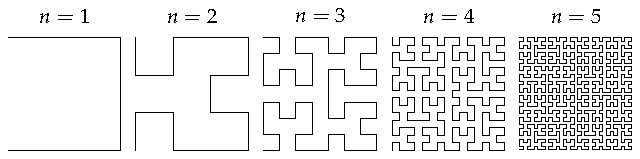
\includegraphics[scale = 1.08]{figures/hilbertcurves}
% \caption{\footnotesize A caption with some text....}
% \end{figure*}

\end{document}